\graphicspath{{../member2/source_figures/}{member2/source_figures/}{source_figures/}}

\subsection*{3a. Tái diễn giải huấn luyện Generative AI qua lăng kính học tăng cường}

Phần này trình bày các nội dung từ Section 2.3 đến Section 2.6 của tutorial \textit{Generative AI Meets Reinforcement Learning}.
Trọng tâm không phải là nhắc lại định nghĩa MDP hay diffusion model cơ bản, mà là phân tích cách các đối tượng quen thuộc của RL, gồm trajectory distribution, score function, policy gradient và reward, có thể được dùng để diễn giải quá trình huấn luyện mô hình sinh.
Cách nhìn này tạo ra hai kết nối song song.
Một mặt, generative models có thể được dùng để biểu diễn policy phức tạp hơn trong RL.
Mặt khác, các estimator và objective của RL có thể được dùng để fine-tune generative models theo các mục tiêu downstream khó biểu diễn bằng likelihood.
Các nội dung được thảo luận gồm phân phối trajectory trong RL, vai trò của score function, diffusion policy trong offline RL, phương pháp Diffusion-DICE, và DDPO như một trường hợp sử dụng RL để fine-tune diffusion model~\citep{eysenbach2025generativerl}.

\subsubsection*{3a.1. Phân phối dữ liệu trong RL và reward-weighted learning}

Trong supervised learning, tập dữ liệu huấn luyện thường được xem như một đại lượng cố định.
Mô hình nhận dataset $\mathcal{D}$ làm đầu vào và tối ưu tham số để khớp nhãn hoặc tăng likelihood trên các mẫu quan sát được.
Ngược lại, trong RL, dữ liệu huấn luyện được sinh ra bởi chính policy đang được tối ưu.
Khi policy thay đổi, tập trajectory quan sát được và phân phối dữ liệu tương ứng cũng thay đổi.
Do đó, bài toán RL không chỉ bao gồm việc tối ưu ánh xạ từ trạng thái sang hành động, mà còn bao gồm việc điều chỉnh phân phối kinh nghiệm do policy tạo ra trong quá trình tương tác.

Gọi $\tau=(s_0,a_0,s_1,a_1,\ldots)$ là một trajectory và $\pi_\theta(\tau)$ là xác suất policy $\pi_\theta$ sinh ra trajectory đó.
Return của trajectory được ký hiệu là $R(\tau)$.
Mục tiêu tối ưu của policy có thể viết dưới dạng:
\begin{equation}
    J(\theta)
    =
    \mathbb{E}_{\tau\sim\pi_\theta}
    \left[
        R(\tau)
    \right].
\end{equation}
Biểu thức này cho thấy chất lượng policy được đánh giá qua kỳ vọng return trên chính các trajectory do policy sinh ra.
Điểm khác biệt quan trọng so với supervised learning nằm ở chỗ phân phối lấy kỳ vọng phụ thuộc vào $\theta$.
Khi policy được cập nhật, phân phối dữ liệu cũng thay đổi theo.

Để phân tích mối quan hệ giữa policy và dữ liệu, có thể đưa vào một phân phối phụ $q(\tau)$ trên trajectory.
Giống như trong lecture notes, ta giả sử return đã được chọn hoặc dịch chuyển sao cho $R(\tau)>0$, để biểu thức $\log R(\tau)$ có nghĩa.
Sử dụng cùng dạng biến đổi với evidence lower bound (ELBO), thu được:
\begin{equation}
    \log \mathbb{E}_{\pi_\theta(\tau)}[R(\tau)]
    =
    \log
    \int
    q(\tau)
    \frac{\pi_\theta(\tau)R(\tau)}{q(\tau)}
    d\tau
    \geq
    \mathbb{E}_{q(\tau)}
    \left[
        \log \pi_\theta(\tau)
        +
        \log R(\tau)
        -
        \log q(\tau)
    \right].
\end{equation}
Lower bound này phụ thuộc đồng thời vào hai đối tượng: policy $\pi_\theta$ và phân phối trajectory $q(\tau)$.
Do đó, cách viết này diễn giải RL như một bài toán tối ưu đồng thời trên policy và phân phối dữ liệu.
Policy cần gán xác suất cao cho các trajectory có chất lượng tốt, trong khi phân phối dữ liệu phụ trợ cần tập trung vào các trajectory có return cao.

Khi tối ưu lower bound theo $q(\tau)$, nghiệm tối ưu có dạng:
\begin{equation}
    q^*(\tau)
    =
    \frac{R(\tau)\pi_\theta(\tau)}
    {\int R(\tau')\pi_\theta(\tau')d\tau'}.
\end{equation}
Phân phối $q^*(\tau)$ là phiên bản được tái trọng số của phân phối trajectory hiện tại.
Các trajectory có return lớn được gán xác suất cao hơn, nhưng vẫn bị ràng buộc bởi hỗ trợ của phân phối trajectory do policy hiện tại sinh ra.
Kết quả này cung cấp một diễn giải xác suất cho reward-weighted regression: dữ liệu huấn luyện có chất lượng cao không được xác định độc lập với policy, mà được hình thành bằng cách tái trọng số dữ liệu do policy sinh ra theo reward~\citep{peters2007rwr}.
Về mặt khái niệm, trajectory đóng vai trò tương tự biến ẩn trong mô hình sinh: ta quan sát được reward mong muốn nhưng không biết trước chuỗi trạng thái--hành động nào sẽ tạo ra reward đó.
Do đó, bài toán tối ưu policy có thể được nhìn như bài toán suy luận trên phân phối trajectory có reward cao.
Đây là điểm làm cho phần 2.3 của tutorial liên hệ trực tiếp với generative modeling: thay vì xem dataset là một đối tượng cố định, RL xem phân phối dữ liệu là một biến cần được cập nhật cùng với policy.

Thay dạng tái trọng số trên vào objective và lấy gradient theo tham số policy dẫn tới dạng policy gradient:
\begin{equation}
    \nabla_\theta J(\theta)
    =
    \mathbb{E}_{\tau\sim\pi_{\mathrm{old}}}
    \left[
        R(\tau)
        \sum_t
        \nabla_\theta
        \log \pi_\theta(a_t\mid s_t)
    \right].
\end{equation}
Công thức này là nền tảng của REINFORCE và các phương pháp policy gradient~\citep{williams1992reinforce}.
Ký hiệu $\pi_{\mathrm{old}}$ nhấn mạnh rằng trong bước cập nhật, trajectory được lấy từ policy ở vòng lặp trước hoặc policy dùng để thu thập batch dữ liệu hiện tại; tham số $\theta$ trong log-likelihood là tham số đang được tối ưu.
Biểu thức này cho thấy sau khi lấy mẫu trajectory, các hành động thuộc những trajectory có return cao sẽ được tăng log-likelihood dưới policy mới.
Theo cách nhìn này, policy improvement có thể được diễn giải như một dạng maximum likelihood có trọng số, trong đó trọng số được xác định bởi reward.
Đây là mối liên hệ trực tiếp giữa tối ưu policy trong RL và huấn luyện mô hình sinh dựa trên likelihood.

\begin{figure}[ht]
    \centering
    \begin{tikzpicture}[
        font=\scriptsize,
        >=Latex,
        box/.style={draw, rounded corners=2pt, align=center, minimum height=0.9cm, minimum width=2.4cm},
        data/.style={box, fill=gray!10},
        process/.style={box, fill=blue!8},
        reward/.style={box, fill=green!10},
        arrow/.style={->, thick}
    ]
        \node[font=\bfseries, anchor=west] at (0,0) {Supervised learning};
        \node[data] (dataset) at (1.7,-0.85) {Dataset cố định\\$\mathcal{D}$};
        \node[process, right=0.9cm of dataset] (sllearn) {Tối ưu\\loss/likelihood};
        \node[data, right=0.9cm of sllearn] (model) {Model\\$p_\theta(x)$};
        \draw[arrow] (dataset) -- (sllearn);
        \draw[arrow] (sllearn) -- (model);

        \node[font=\bfseries, anchor=west] at (0,-2.65) {Reinforcement learning};
        \node[data] (policy) at (1.7,-3.55) {Policy\\$\pi_\theta$};
        \node[data, right=0.75cm of policy] (traj) {Trajectory\\$\tau\sim\pi_\theta$};
        \node[reward, right=0.75cm of traj] (return) {Return\\$R(\tau)$};
        \node[data, below=0.8cm of traj] (qstar) {Dữ liệu tái trọng số\\$q^*(\tau)\propto R(\tau)\pi_\theta(\tau)$};
        \node[process, left=0.75cm of qstar] (rlearn) {Policy\\improvement};

        \draw[arrow] (policy) -- (traj);
        \draw[arrow] (traj) -- (return);
        \draw[arrow] (return) |- (qstar);
        \draw[arrow] (qstar) -- (rlearn);
        \draw[arrow] (rlearn) -- (policy);
    \end{tikzpicture}
    \caption{Sơ đồ tóm tắt quan điểm tối ưu đồng thời policy và phân phối experience trong RL. Trajectory có reward cao được tái trọng số và trở thành dữ liệu huấn luyện cho bước policy improvement. Dựa trên Eysenbach \& Zhang, ICML tutorial notes~\citep{eysenbach2025generativerl}.}
    \label{fig:tv2-notes-fig5-6}
\end{figure}

\subsubsection*{3a.2. Score function và mô hình sinh làm policy}

Trong biểu thức policy gradient, số hạng cốt lõi là:
\begin{equation}
    \nabla_\theta \log \pi_\theta(a_t\mid s_t).
\end{equation}
Đây là score function của policy theo tham số $\theta$.
Trong RL, score function xác định hướng thay đổi tham số nhằm tăng xác suất của các hành động gắn với return cao.
Trong generative modeling, log-probability và score function cũng là các đại lượng trung tâm, đặc biệt trong score-based diffusion models.
Sự tương ứng này cho phép diễn giải policy như một mô hình sinh hành động có điều kiện theo trạng thái~\citep{eysenbach2025generativerl}.

Nếu policy được mô hình hóa bằng Gaussian đơn mode, không gian hành động được biểu diễn tương đối hạn chế.
Tuy nhiên, công thức policy gradient không bắt buộc policy phải thuộc một họ phân phối đơn giản.
Các kiến trúc như transformer, diffusion model hoặc flow-based model đều có thể đóng vai trò policy nếu chúng cung cấp được log-probability hoặc score cần thiết cho quá trình tối ưu.
Nói cách khác, Gaussian policy trong các ví dụ RL cổ điển chỉ là một lựa chọn tham số hóa thuận tiện, không phải điều kiện bắt buộc của lập luận toán học.
Với transformer policy, score có thể được tính từ log-probability của action token hoặc action sequence; với diffusion policy, score có thể đến từ denoising score hoặc likelihood của transition trong quá trình sampling.
Điểm then chốt của Section 2.4 là khả năng thay policy đơn giản bằng một mô hình sinh giàu khả năng biểu diễn, miễn là thuật toán vẫn truy cập được đại lượng score phù hợp để đưa vào policy-gradient update~\citep{eysenbach2025generativerl}.
Do đó, generative modeling không chỉ đóng vai trò công cụ phụ trợ cho RL, mà còn có thể trực tiếp mở rộng lớp policy được sử dụng trong các thuật toán RL.

Một trường hợp đại diện là reward-conditioned sequence modeling.
Thay vì học policy không điều kiện $\pi(a\mid s)$, mô hình học phân phối:
\begin{equation}
    \pi(a\mid s, R_{\text{target}}),
\end{equation}
trong đó $R_{\text{target}}$ là return mong muốn.
Decision Transformer biểu diễn trajectory thành chuỗi return-to-go, state và action, sau đó dùng transformer tự hồi quy để dự đoán action kế tiếp~\citep{chen2021decision}.
Cách tiếp cận này chuyển bài toán điều khiển thành bài toán sinh chuỗi có điều kiện.
Khi được điều kiện hóa bởi return-to-go cao, mô hình được kỳ vọng sinh ra các hành động tương tự những đoạn trajectory đạt return cao trong dữ liệu.
Điểm khác biệt với behavioral cloning thông thường là biến điều kiện $R_{\text{target}}$ đóng vai trò chỉ định mức chất lượng mong muốn của hành vi.
Nếu behavioral cloning chỉ học trung bình hành vi trong dataset, reward-conditioned modeling cố gắng tách các hành vi theo mức return và truy vấn mô hình ở vùng return cao.
Theo ngôn ngữ của mô hình sinh, đây là một dạng conditional generation trên trajectory: prompt của mô hình không phải chỉ là state hiện tại, mà còn là mức return mà ta muốn trajectory đạt được.
Tuy nhiên, vì mô hình vẫn được huấn luyện trên offline dataset, hiệu quả của phương pháp phụ thuộc đáng kể vào coverage của dữ liệu.
Nếu dataset không chứa đủ hành vi chất lượng cao hoặc môi trường có mức ngẫu nhiên lớn, việc điều kiện hóa trên return mong muốn chưa bảo đảm tạo ra năng lực exploration mới~\citep{paster2022luck}.

Trong các bài toán hành động liên tục hoặc đa mode, diffusion policy là một lớp policy linh hoạt hơn.
Một diffusion behavior policy $\pi^D(a\mid s)$ có thể biểu diễn nhiều mode hành động hợp lệ tại cùng một trạng thái.
Để đưa tín hiệu reward hoặc critic vào quá trình lựa chọn hành động, các phương pháp diffusion policy thường được phân thành hai nhóm.

Nhóm \textbf{guide-based} thay đổi quá trình denoising bằng một guidance term.
Sau khi huấn luyện behavior diffusion policy, score của policy được tăng cường theo dạng:
\begin{equation}
    \nabla_{a_t}\log \pi_t(a_t\mid s)
    =
    \nabla_{a_t}\log \pi_t^D(a_t\mid s)
    +
    \nabla_{a_t}J_t(a_t).
\end{equation}
Trong đó, $\pi_t^D$ là behavior policy tại diffusion timestep $t$, còn $J_t$ là guidance term được học từ reward hoặc critic.
Các phương pháp như Diffuser và QGPO thuộc hướng này~\citep{janner2022diffuser,lu2023qgpo}.

Nhóm \textbf{select-based} giữ nguyên cơ chế sinh ứng viên của diffusion policy, sau đó chọn action dựa trên critic.
Giả sử diffusion policy sinh ra tập ứng viên $\{a_0^i\}_{i=1}^{N}$, xác suất chọn ứng viên thứ $j$ có thể viết:
\begin{equation}
    \Pr[a=a_0^j\mid s]
    =
    \frac{w(s,a_0^j)}
    {\sum_{i=1}^{N} w(s,a_0^i)}.
\end{equation}
Ở đây $w(s,a_0^j)$ là trọng số được tính từ critic hoặc hàm giá trị.
IDQL là một ví dụ của hướng select-based sử dụng diffusion policy trong actor-critic offline RL~\citep{hansenestruch2023idql}.

\begin{figure}[ht]
    \centering
    \begin{tikzpicture}[
        font=\small,
        >=Latex,
        box/.style={draw, rounded corners=2pt, align=center, minimum height=0.8cm, text width=2.25cm},
        behavior/.style={box, fill=gray!10},
        guide/.style={box, fill=blue!8},
        select/.style={box, fill=green!10},
        risk/.style={box, fill=red!8},
        arrow/.style={->, thick}
    ]
        \node[behavior] (data) {Offline dataset\\$\mathcal{D}$};
        \node[behavior, right=0.55cm of data] (diff) {Diffusion behavior\\$\pi^D(a\mid s)$};

        \node[guide, right=0.75cm of diff, yshift=1.65cm] (guideonly) {Guide-based\\augmented score};
        \node[risk, right=0.55cm of guideonly] (ood1) {Có thể drift\\sang OOD actions};

        \node[select, right=0.75cm of diff] (selectonly) {Select-based\\candidate ranking};
        \node[risk, right=0.55cm of selectonly] (ood2) {Critic có thể\\overestimate OOD};

        \node[guide, right=0.75cm of diff, yshift=-1.65cm] (diceguide) {Diffusion-DICE\\Guide};
        \node[select, right=0.55cm of diceguide] (diceselect) {Then Select\\in-sample candidates};
        \node[behavior, right=0.55cm of diceselect] (action) {Action chọn\\ít error exploitation};

        \draw[arrow] (data) -- (diff);
        \draw[arrow] (diff) -- (guideonly);
        \draw[arrow] (guideonly) -- (ood1);
        \draw[arrow] (diff) -- (selectonly);
        \draw[arrow] (selectonly) -- (ood2);
        \draw[arrow] (diff) -- (diceguide);
        \draw[arrow] (diceguide) -- (diceselect);
        \draw[arrow] (diceselect) -- (action);
    \end{tikzpicture}
    \caption{Sơ đồ tự vẽ tóm tắt quan hệ giữa guide-based, select-based và Guide-Then-Select trong Diffusion-DICE. Sơ đồ dựa trên mô tả ở Section 2.5 của tutorial và abstract Diffusion-DICE~\citep{eysenbach2025generativerl,mao2024diffusiondice}.}
    \label{fig:tv2-guide-select-tikz}
\end{figure}

Một hạn chế chung của guide-based và select-based là sự phụ thuộc vào critic.
Trong offline RL, critic chỉ được huấn luyện trên dataset cố định.
Khi diffusion policy sinh ra action nằm ngoài phân phối dữ liệu, critic có thể đánh giá sai và overestimate giá trị của action đó.
Nếu policy tối ưu hóa theo các dự đoán sai này, nó có thể khuếch đại lỗi ngoại suy thay vì tìm được hành động có reward thực sự cao.
Hiện tượng này được gọi là value error exploitation.
Hình~\ref{fig:tv2-notes-fig7} minh họa hiện tượng này trong toycase của Diffusion-DICE.

\subsubsection*{3a.3. Diffusion-DICE trong offline RL}

Diffusion-DICE được đề xuất cho bối cảnh offline RL, nơi agent chỉ có một dataset cố định và không thể tương tác thêm với môi trường trong quá trình học~\citep{mao2024diffusiondice}.
Trong thiết lập này, diffusion policy có lợi thế vì nó có khả năng khớp phân phối hành động phức tạp của behavior policy.
Tuy nhiên, khả năng sinh mẫu đa dạng cũng làm tăng nguy cơ xuất hiện action nằm ngoài vùng dữ liệu đáng tin cậy.
Nếu critic đánh giá cao các action ngoài phân phối do lỗi ngoại suy, policy có thể dịch chuyển về các vùng có giá trị ước lượng cao nhưng reward thực thấp.

Ý tưởng trung tâm của Diffusion-DICE là kết hợp hai giai đoạn guide và select trong một paradigm thống nhất.
Về mặt lý thuyết, score của policy tối ưu có thể được phân rã thành score của behavior policy và một thành phần guidance liên quan đến tỷ số phân phối tối ưu.
Gọi $d^*(s,a_0)$ là optimal state-action distribution và $d^D(s,a_0)$ là distribution của behavior policy trong dataset offline.
Về mặt toán học, thành phần guidance tại diffusion timestep $t$ liên quan đến log-density-ratio giữa optimal distribution $d^*$ và behavior distribution $d^D$.
Trong bài báo Diffusion-DICE, second term này có dạng gradient của một log-expectation theo $a_0$, nhưng không được tính trực tiếp vì kỳ vọng điều kiện này thường intractable.
Do đó, Diffusion-DICE đề xuất một biến đổi toán học để chuyển việc học guidance thành một convex optimization problem có thể ước lượng hoàn toàn bằng các mẫu in-sample, tránh việc đánh giá các action nằm ngoài phân phối dữ liệu~\citep{mao2024diffusiondice}.
Trong phần dưới, ký hiệu $G_t(a_t,s)$ được dùng để chỉ learned guidance potential tại diffusion timestep $t$, không phải một closed-form term có thể tính trực tiếp.
Khi đó, score của policy tối ưu được diễn giải dưới dạng:
\begin{equation}
    \nabla_{a_t}\log \pi_t^*(a_t\mid s)
    =
    \underbrace{\nabla_{a_t}\log \pi_t^D(a_t\mid s)}_{\text{behavior score}}
    +
    \underbrace{\nabla_{a_t}G_t(a_t,s)}_{\text{in-sample guidance}}.
\end{equation}
Thành phần behavior score duy trì quá trình sinh mẫu gần với phân phối dữ liệu offline.
Thành phần guidance định hướng mẫu về phía các vùng tương ứng với optimal distribution.
Điểm then chốt là guidance được học theo hướng in-sample, qua đó giảm sự phụ thuộc vào khả năng ngoại suy của critic tại các vùng chưa được quan sát.

Quy trình Guide-Then-Select gồm hai bước.
Trong bước Guide, mô hình sử dụng behavior score kết hợp với learned in-sample guidance để sinh một tập ứng viên hành động.
Bước này cho phép bao phủ nhiều mode khác nhau của policy tối ưu, thay vì hội tụ sớm vào một mode cục bộ.
Trong bước Select, Q-function được sử dụng để chọn action tốt nhất trong số các ứng viên đã sinh.
Do bước select chỉ so sánh trong tập ứng viên được tạo ra bởi guided diffusion, critic ít phải đánh giá các action ở quá xa phân phối dữ liệu.
Sự kết hợp này giúp giảm value error exploitation so với các phương pháp chỉ dùng guide hoặc chỉ dùng select.

Thí nghiệm toycase 2D bandit trong tutorial minh họa trực quan hiện tượng trên.
Offline action dataset nằm trong một annular region.
Ground-truth reward có các đỉnh hướng ra outer circle, trong khi reward model học từ dữ liệu có thể overestimate ở vùng inner circle do thiếu coverage.
Các phương pháp guide-only hoặc select-only có xu hướng dịch chuyển vào vùng inner circle có giá trị ước lượng sai.
Diffusion-DICE, nhờ kết hợp guide-then-select và cơ chế in-sample, sinh action hướng tới vùng outer circle có reward thực cao hơn.
Kết quả này cho thấy vai trò của việc kiểm soát distribution shift trong diffusion-based offline RL.

\begin{figure}[ht]
    \centering
    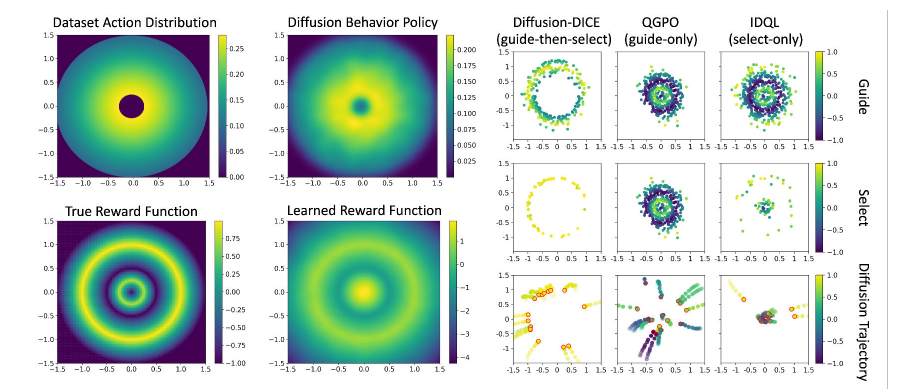
\includegraphics[width=0.98\textwidth]{notes_fig7_plot.png}
    \caption{Toycase 2D bandit minh họa value error exploitation: offline action distribution nằm trong annular region, reward thật đạt giá trị cao ở outer circle, trong khi một số phương pháp bị hút vào vùng inner circle do critic overestimate. Nguồn: Eysenbach \& Zhang, ICML tutorial notes~\citep{eysenbach2025generativerl}.}
    \label{fig:tv2-notes-fig7}
\end{figure}

\subsubsection*{3a.4. DDPO: tối ưu diffusion model bằng RL}

Các nội dung trước cho thấy generative models có thể được sử dụng như policy trong RL.
Chiều ngược lại là sử dụng RL để tối ưu chính generative model theo mục tiêu downstream.
DDPO (\textit{Denoising Diffusion Policy Optimization}) là một trường hợp tiêu biểu cho hướng tiếp cận này.
Thay vì chỉ huấn luyện diffusion model bằng denoising score matching hoặc objective xấp xỉ likelihood, DDPO tối ưu model theo reward được định nghĩa trên mẫu cuối, chẳng hạn aesthetic quality, compressibility hoặc prompt-image alignment~\citep{black2024ddpo}.

Ý tưởng cơ bản của DDPO là mô hình hóa quá trình denoising như một multi-step MDP.
Tại diffusion timestep $t$, state gồm noisy sample $x_t$ và context/prompt $c$.
Policy là phân phối chuyển tiếp của diffusion model:
\begin{equation}
    p_\theta(x_{t-1}\mid x_t,c).
\end{equation}
Một action trong MDP tương ứng với việc lấy mẫu bước denoising kế tiếp $x_{t-1}$ từ phân phối này.
Do đó, đối tượng tối ưu không chỉ là output cuối cùng $x_0$, mà là toàn bộ chuỗi quyết định denoising tạo ra $x_0$.

Trajectory của quá trình sinh mẫu được viết:
\begin{equation}
    x_T \rightarrow x_{T-1} \rightarrow \cdots \rightarrow x_0.
\end{equation}
Reward được tính ở mẫu cuối $x_0$:
\begin{equation}
    \max_\theta
    \mathbb{E}_{c\sim p(c),\,\tau\sim p_\theta(\tau\mid c)}
    \left[
        r(x_0,c)
    \right].
\end{equation}
Vì xác suất trajectory phân rã qua nhiều transition denoising, policy gradient có dạng:
\begin{equation}
    \nabla_\theta J(\theta)
    =
    \mathbb{E}_{c\sim p(c),\,\tau\sim p_\theta(\tau\mid c)}
    \left[
        r(x_0,c)
        \sum_{t=1}^{T}
        \nabla_\theta
        \log p_\theta(x_{t-1}\mid x_t,c)
    \right].
\end{equation}
Công thức này cho phép lan truyền tín hiệu reward cuối tới từng bước denoising thông qua log-probability của transition.
Do đó, diffusion sampling được chuyển thành một bài toán sequential decision-making có thể tối ưu bằng policy gradient.
Trong bài báo DDPO, hai estimator chính được xét là DDPO-SF và DDPO-IS.
DDPO-SF dùng score-function estimator trực tiếp trên trajectory denoising, tương tự REINFORCE.
DDPO-IS bổ sung importance sampling và cơ chế clipping theo tinh thần PPO để có thể dùng lại batch trajectory được sinh bởi policy cũ trong nhiều bước cập nhật.
Sự khác biệt này có ý nghĩa thực nghiệm vì sinh ảnh bằng diffusion model tốn chi phí cao; nếu mỗi batch chỉ được dùng một lần, hiệu quả sử dụng mẫu sẽ thấp.
Do đó, DDPO-IS thường là biến thể thực dụng hơn trong các thí nghiệm text-to-image fine-tuning của bài báo~\citep{black2024ddpo}.

DDPO cũng làm rõ hạn chế của reward-weighted regression khi áp dụng trực tiếp cho diffusion model.
RWR xem toàn bộ quá trình sinh ảnh như một quyết định một bước: model sinh mẫu cuối, reward được tính, và các mẫu có reward cao được tăng trọng số trong objective huấn luyện.
Tuy nhiên, objective DDPM thường là một variational bound hoặc xấp xỉ likelihood, không phải exact log-likelihood của $p_\theta(x_0\mid c)$~\citep{black2024ddpo}.
Vì vậy, việc reweight mẫu cuối chỉ tối ưu downstream objective một cách gián tiếp và xấp xỉ.
Một hạn chế thứ hai là credit assignment: RWR chỉ quan sát reward của $x_0$ và tăng trọng số cho toàn bộ mẫu cuối, nên không mô hình hóa rõ transition denoising nào trong chuỗi $x_T\rightarrow\cdots\rightarrow x_0$ đã đóng góp vào reward đó.
Trong khung MDP của DDPO, mỗi bước $x_t\rightarrow x_{t-1}$ là một decision có log-probability riêng; vì vậy cùng một reward cuối $r(x_0,c)$ được phân bổ vào gradient của từng transition xuất hiện trên trajectory.
DDPO giữ lại cấu trúc nhiều bước của denoising process và dùng likelihood của từng transition $p_\theta(x_{t-1}\mid x_t,c)$, nhờ đó tạo được các Monte Carlo policy-gradient estimates trực tiếp hơn trên trajectory denoising~\citep{black2024ddpo}.

Ý nghĩa của DDPO nằm ở việc đưa reward-based optimization vào diffusion model theo một cấu trúc ra quyết định tuần tự.
Phương pháp này cho phép fine-tune model theo các tiêu chí khó biểu diễn bằng likelihood, nhưng có thể được đánh giá bằng reward model hoặc hàm đánh giá black-box.
Đồng thời, phương pháp cũng đặt ra các giới hạn cần xem xét: nếu reward model không phản ánh đúng chất lượng mong muốn, diffusion model có thể khai thác reward thay vì cải thiện chất lượng thực.
Do đó, trong giao thoa giữa generative AI và RL, thiết kế reward và kiểm soát distribution shift là các vấn đề quan trọng không kém việc xây dựng lớp policy biểu diễn mạnh.

\subsubsection*{3a.5. Nhận xét chung}

Các phân tích trên cho thấy mối quan hệ giữa generative AI và RL không chỉ nằm ở việc sử dụng một mô hình sinh mạnh hơn để thay thế policy truyền thống.
Ở mức toán học, score function và log-probability tạo ra một ngôn ngữ chung cho hai lĩnh vực.
Ở mức thuật toán, reward-weighted learning, diffusion policy, Diffusion-DICE và DDPO đều khai thác quan hệ giữa phân phối dữ liệu, likelihood và reward.
Tuy nhiên, các phương pháp này cũng chia sẻ một rủi ro chung: khi critic hoặc reward model sai lệch, quá trình tối ưu có thể khuếch đại sai số.
Điểm này xuất hiện ở cả hai phía của mối liên hệ.
Trong offline RL, diffusion policy có thể sinh action ngoài phân phối dữ liệu và làm critic overestimate.
Trong RL fine-tuning diffusion model, reward model có thể trở thành một proxy bị khai thác quá mức.
Vì vậy, các hướng nghiên cứu tiếp theo cần kết hợp mô hình sinh giàu khả năng biểu diễn với cơ chế đánh giá reward đáng tin cậy, kiểm soát ngoại suy, và phân tích rõ hơn tác động của distribution shift trong quá trình học.
Một kết luận quan trọng từ phần này là khả năng biểu diễn mạnh của generative models chỉ giải quyết một phần bài toán.
Để xây dựng hệ thống RL--GenAI ổn định, cần đồng thời xử lý ba vấn đề: dữ liệu do policy sinh ra có phân phối thay đổi, reward hoặc critic có thể sai ở vùng ít dữ liệu, và objective tối ưu có thể khác đáng kể so với likelihood training ban đầu.
